%%%%%%%%%%%%%%%%%%%%%%%%%%%%%%%%%%%%%%%%%%%%%%%%%%%%%%%%%%%%%%%%%%%%%%%%%%
%DIF LATEXDIFF DIFFERENCE FILE
%DIF DEL dm-template.tex                Sun Jun  3 10:50:23 2018
%DIF ADD AfterReviews/dm-template.tex   Sun Jun  3 10:50:23 2018
%
% 	Template for seminar reports
%
%%%%%%%%%%%%%%%%%%%%%%%%%%%%%%%%%%%%%%%%%%%%%%%%%%%%%%%%%%%%%%%%%%%%%%%%%%

%%%%%%%%%%%%%%%%%%%%%%%%%%%%%%%%%%%%%%%%%%%%%%%%%%%%%%%%%%%%%%%%%%%%%%%%%%
% 	Include layout and macros
%%%%%%%%%%%%%%%%%%%%%%%%%%%%%%%%%%%%%%%%%%%%%%%%%%%%%%%%%%%%%%%%%%%%%%%%%%


%% This LaTeX template is based on the following example file included in the ieeetran
%% package:
%% bare_conf.tex 
%% V1.2
%% 2002/11/18
%% by Michael Shell
%% mshell@ece.gatech.edu
%% (requires IEEEtran.cls version 1.6b or later) with an IEEE conference paper.


% Note that the a4paper option is mainly intended so that authors in
% countries using A4 can easily print to A4 and see how their papers will
% look in print. Authors are encouraged to use U.S. letter paper when 
% submitting to IEEE. Use the testflow package mentioned above to verify
% correct handling of both paper sizes by the author's LaTeX system.
%
% Also note that the "draftcls" or "draftclsnofoot", not "draft", option
% should be used if it is desired that the figures are to be displayed in
% draft mode.
%
% This paper can be formatted using the peerreviewca
% (instead of conference) mode.
\documentclass[conference, a4paper]{IEEEtran-modified}
% If the IEEEtran.cls has not been installed into the LaTeX system files, 
% manually specify the path to it:
% \documentclass[conference]{../sty/IEEEtran} 

\IEEEoverridecommandlockouts

% some very useful LaTeX packages include:

\usepackage{cite}       % Written by Donald Arseneau
                        % V1.6 and later of IEEEtran pre-defines the format
                        % of the cite.sty package \cite{} output to follow
                        % that of IEEE. Loading the cite package will
                        % result in citation numbers being automatically
                        % sorted and properly "ranged". i.e.,
                        % [1], [9], [2], [7], [5], [6]
                        % (without using cite.sty)
                        % will become:
                        % [1], [2], [5]--[7], [9] (using cite.sty)
                        % cite.sty's \cite will automatically add leading
                        % space, if needed. Use cite.sty's noadjust option
                        % (cite.sty V3.8 and later) if you want to turn this
                        % off. cite.sty is already installed on most LaTeX
                        % systems. The latest version can be obtained at:
                        % http://www.ctan.org/tex-archive/macros/latex/contrib/supported/cite/

%\usepackage{graphicx}  % Written by David Carlisle and Sebastian Rahtz
                        % Required if you want graphics, photos, etc.
                        % graphicx.sty is already installed on most LaTeX
                        % systems. The latest version and documentation can
                        % be obtained at:
                        % http://www.ctan.org/tex-archive/macros/latex/required/graphics/
                        % Another good source of documentation is "Using
                        % Imported Graphics in LaTeX2e" by Keith Reckdahl
                        % which can be found as esplatex.ps and epslatex.pdf
                        % at: http://www.ctan.org/tex-archive/info/
% NOTE: for dual use with latex and pdflatex, instead load graphicx like:
\ifx\pdfoutput\undefined
	\usepackage{graphicx}
\else
	\usepackage[pdftex]{graphicx}
\fi

% However, be warned that pdflatex will require graphics to be in PDF
% (not EPS) format and will preclude the use of PostScript based LaTeX
% packages such as psfrag.sty and pstricks.sty. IEEE conferences typically
% allow PDF graphics (and hence pdfLaTeX). However, IEEE journals do not
% (yet) allow image formats other than EPS or TIFF. Therefore, authors of
% journal papers should use traditional LaTeX with EPS graphics.
%
% The path(s) to the graphics files can also be declared: e.g.,
% \graphicspath{{../eps/}{../ps/}}
% if the graphics files are not located in the same directory as the
% .tex file. This can be done in each branch of the conditional above
% (after graphicx is loaded) to handle the EPS and PDF cases separately.
% In this way, full path information will not have to be specified in
% each \includegraphics command.
%
% Note that, when switching from latex to pdflatex and vice-versa, the new
% compiler will have to be run twice to clear some warnings.
\graphicspath{{figures/}}


%\usepackage{psfrag}    % Written by Craig Barratt, Michael C. Grant,
                        % and David Carlisle
                        % This package allows you to substitute LaTeX
                        % commands for text in imported EPS graphic files.
                        % In this way, LaTeX symbols can be placed into
                        % graphics that have been generated by other
                        % applications. You must use latex->dvips->ps2pdf
                        % workflow (not direct pdf output from pdflatex) if
                        % you wish to use this capability because it works
                        % via some PostScript tricks. Alternatively, the
                        % graphics could be processed as separate files via
                        % psfrag and dvips, then converted to PDF for
                        % inclusion in the main file which uses pdflatex.
                        % Docs are in "The PSfrag System" by Michael C. Grant
                        % and David Carlisle. There is also some information 
                        % about using psfrag in "Using Imported Graphics in
                        % LaTeX2e" by Keith Reckdahl which documents the
                        % graphicx package (see above). The psfrag package
                        % and documentation can be obtained at:
                        % http://www.ctan.org/tex-archive/macros/latex/contrib/supported/psfrag/

%\usepackage{subfigure} % Written by Steven Douglas Cochran
                        % This package makes it easy to put subfigures
                        % in your figures. i.e., "figure 1a and 1b"
                        % Docs are in "Using Imported Graphics in LaTeX2e"
                        % by Keith Reckdahl which also documents the graphicx
                        % package (see above). subfigure.sty is already
                        % installed on most LaTeX systems. The latest version
                        % and documentation can be obtained at:
                        % http://www.ctan.org/tex-archive/macros/latex/contrib/supported/subfigure/

\usepackage{url}       % Written by Donald Arseneau
                        % Provides better support for handling and breaking
                        % URLs. url.sty is already installed on most LaTeX
                        % systems. The latest version can be obtained at:
                        % http://www.ctan.org/tex-archive/macros/latex/contrib/other/misc/
                        % Read the url.sty source comments for usage information.

%\usepackage{stfloats}  % Written by Sigitas Tolusis
                        % Gives LaTeX2e the ability to do double column
                        % floats at the bottom of the page as well as the top.
                        % (e.g., "\begin{figure*}[!b]" is not normally
                        % possible in LaTeX2e). This is an invasive package
                        % which rewrites many portions of the LaTeX2e output
                        % routines. It may not work with other packages that
                        % modify the LaTeX2e output routine and/or with other
                        % versions of LaTeX. The latest version and
                        % documentation can be obtained at:
                        % http://www.ctan.org/tex-archive/macros/latex/contrib/supported/sttools/
                        % Documentation is contained in the stfloats.sty
                        % comments as well as in the presfull.pdf file.
                        % Do not use the stfloats baselinefloat ability as
                        % IEEE does not allow \baselineskip to stretch.
                        % Authors submitting work to the IEEE should note
                        % that IEEE rarely uses double column equations and
                        % that authors should try to avoid such use.
                        % Do not be tempted to use the cuted.sty or
                        % midfloat.sty package (by the same author) as IEEE
                        % does not format its papers in such ways.

\usepackage{amsmath}    % From the American Mathematical Society
\usepackage{amssymb}
                        % A popular package that provides many helpful commands
                        % for dealing with mathematics. Note that the AMSmath
                        % package sets \interdisplaylinepenalty to 10000 thus
                        % preventing page breaks from occurring within multiline
                        % equations. Use:
\interdisplaylinepenalty=2500
                        % after loading amsmath to restore such page breaks
                        % as IEEEtran.cls normally does. amsmath.sty is already
                        % installed on most LaTeX systems. The latest version
                        % and documentation can be obtained at:
                        % http://www.ctan.org/tex-archive/macros/latex/required/amslatex/math/

%My packages
\usepackage{todonotes}
\usepackage{pgfplots}
\usepackage{bm}
\usepackage{soul}
\usepackage{lipsum}
\usepackage{verbatim}
\usepackage{algorithm}
\usepackage{algpseudocode}
\DeclareMathOperator{\sign}{sign}
\DeclareMathOperator{\softmax}{softmax}
\newcommand{\nth}[1]{$#1^\text{th}$}
\newcommand{\given}{\,|\,}
\DeclareMathOperator*{\argmax}{arg\,max}
\DeclareMathOperator{\loss}{\mathcal{L}}
% \relpenalty=9999

% Other popular packages for formatting tables and equations include:

%\usepackage{array}
% Frank Mittelbach's and David Carlisle's array.sty which improves the
% LaTeX2e array and tabular environments to provide better appearances and
% additional user controls. array.sty is already installed on most systems.
% The latest version and documentation can be obtained at:
% http://www.ctan.org/tex-archive/macros/latex/required/tools/

% Mark Wooding's extremely powerful MDW tools, especially mdwmath.sty and
% mdwtab.sty which are used to format equations and tables, respectively.
% The MDWtools set is already installed on most LaTeX systems. The lastest
% version and documentation is available at:
% http://www.ctan.org/tex-archive/macros/latex/contrib/supported/mdwtools/


% V1.6 of IEEEtran contains the IEEEeqnarray family of commands that can
% be used to generate multiline equations as well as matrices, tables, etc.


% Also of notable interest:

% Scott Pakin's eqparbox package for creating (automatically sized) equal
% width boxes. Available:
% http://www.ctan.org/tex-archive/macros/latex/contrib/supported/eqparbox/



% Notes on hyperref:
% IEEEtran.cls attempts to be compliant with the hyperref package, written
% by Heiko Oberdiek and Sebastian Rahtz, which provides hyperlinks within
% a document as well as an index for PDF files (produced via pdflatex).
% However, it is a tad difficult to properly interface LaTeX classes and
% packages with this (necessarily) complex and invasive package. It is
% recommended that hyperref not be used for work that is to be submitted
% to the IEEE. Users who wish to use hyperref *must* ensure that their
% hyperref version is 6.72u or later *and* IEEEtran.cls is version 1.6b 
% or later. The latest version of hyperref can be obtained at:
%
% http://www.ctan.org/tex-archive/macros/latex/contrib/supported/hyperref/
%
% Also, be aware that cite.sty (as of version 3.9, 11/2001) and hyperref.sty
% (as of version 6.72t, 2002/07/25) do not work optimally together.
% To mediate the differences between these two packages, IEEEtran.cls, as
% of v1.6b, predefines a command that fools hyperref into thinking that
% the natbib package is being used - causing it not to modify the existing
% citation commands, and allowing cite.sty to operate as normal. However,
% as a result, citation numbers will not be hyperlinked. Another side effect
% of this approach is that the natbib.sty package will not properly load
% under IEEEtran.cls. However, current versions of natbib are not capable
% of compressing and sorting citation numbers in IEEE's style - so this
% should not be an issue. If, for some strange reason, the user wants to
% load natbib.sty under IEEEtran.cls, the following code must be placed
% before natbib.sty can be loaded:
%
% \makeatletter
% \let\NAT@parse\undefined
% \makeatother
%
% Hyperref should be loaded differently depending on whether pdflatex
% or traditional latex is being used:
%
%\ifx\pdfoutput\undefined
%\usepackage[hypertex]{hyperref}
%\else
%\usepackage[pdftex,hypertexnames=false]{hyperref}
%\fi
%
% Pdflatex produces superior hyperref results and is the recommended
% compiler for such use.



% *** Do not adjust lengths that control margins, column widths, etc. ***
% *** Do not use packages that alter fonts (such as pslatex).         ***
% There should be no need to do such things with IEEEtran.cls V1.6 and later.


%%%%%%%%%%%%%%%%%%%%%%%%%%%%%%%%%%%%%%%%%%%%%%%%%%%%%%%%%%%%%%%%%%%%%%%%%%
% 	Anpassung an deutsche Texte
%%%%%%%%%%%%%%%%%%%%%%%%%%%%%%%%%%%%%%%%%%%%%%%%%%%%%%%%%%%%%%%%%%%%%%%%%%

%\usepackage{ngerman}
\usepackage[latin1]{inputenc}   % f�r Umlaute 

%\renewcommand{\abstractname}{Kurzfassung}      % statt Zusammenfassung, wie es ngerman definiert
%\renewcommand{\keywordname}{Schl�sselworte}
%\renewcommand{\figurename}{Abb.}




%%%%%%%%%%%%%%%%%%%%%%%%%%%%%%%%%%%%%%%%%%%%%%%%%%%%%%%%%%%%%%%%%%%%%%%%%%
% 	Page numbering (not on first page)
%%%%%%%%%%%%%%%%%%%%%%%%%%%%%%%%%%%%%%%%%%%%%%%%%%%%%%%%%%%%%%%%%%%%%%%%%%
\pagestyle{empty}

%%%%%%%%%%%%%%%%%%%%%%%%%%%%%%%%%%%%%%%%%%%%%%%%%%%%%%%%%%%%%%%%%%%%%%%%%%
% 	Correct bad hyphenation here
%%%%%%%%%%%%%%%%%%%%%%%%%%%%%%%%%%%%%%%%%%%%%%%%%%%%%%%%%%%%%%%%%%%%%%%%%%

\hyphenation{}

%%%%%%%%%%%%%%%%%%%%%%%%%%%%%%%%%%%%%%%%%%%%%%%%%%%%%%%%%%%%%%%%%%%%%%%%%%
% 	Begin of the document
%%%%%%%%%%%%%%%%%%%%%%%%%%%%%%%%%%%%%%%%%%%%%%%%%%%%%%%%%%%%%%%%%%%%%%%%%%
%DIF PREAMBLE EXTENSION ADDED BY LATEXDIFF
%DIF UNDERLINE PREAMBLE %DIF PREAMBLE
\RequirePackage[normalem]{ulem} %DIF PREAMBLE
\RequirePackage{color}\definecolor{RED}{rgb}{1,0,0}\definecolor{BLUE}{rgb}{0,0,1} %DIF PREAMBLE
\providecommand{\DIFadd}[1]{{\protect\color{blue}\uwave{#1}}} %DIF PREAMBLE
\providecommand{\DIFdel}[1]{{\protect\color{red}\sout{#1}}}                      %DIF PREAMBLE
%DIF SAFE PREAMBLE %DIF PREAMBLE
\providecommand{\DIFaddbegin}{} %DIF PREAMBLE
\providecommand{\DIFaddend}{} %DIF PREAMBLE
\providecommand{\DIFdelbegin}{} %DIF PREAMBLE
\providecommand{\DIFdelend}{} %DIF PREAMBLE
%DIF FLOATSAFE PREAMBLE %DIF PREAMBLE
\providecommand{\DIFaddFL}[1]{\DIFadd{#1}} %DIF PREAMBLE
\providecommand{\DIFdelFL}[1]{\DIFdel{#1}} %DIF PREAMBLE
\providecommand{\DIFaddbeginFL}{} %DIF PREAMBLE
\providecommand{\DIFaddendFL}{} %DIF PREAMBLE
\providecommand{\DIFdelbeginFL}{} %DIF PREAMBLE
\providecommand{\DIFdelendFL}{} %DIF PREAMBLE
%DIF END PREAMBLE EXTENSION ADDED BY LATEXDIFF

\begin{document}

%%%%%%%%%%%%%%%%%%%%%%%%%%%%%%%%%%%%%%%%%%%%%%%%%%%%%%%%%%%%%%%%%%%%%%%%%%
% 	Paper title
%%%%%%%%%%%%%%%%%%%%%%%%%%%%%%%%%%%%%%%%%%%%%%%%%%%%%%%%%%%%%%%%%%%%%%%%%%

\title{Fundamentals of Neural Networks}

%%%%%%%%%%%%%%%%%%%%%%%%%%%%%%%%%%%%%%%%%%%%%%%%%%%%%%%%%%%%%%%%%%%%%%%%%%
% 	Author names and affiliations 
%		-	multiple columns for up to three different affilitations are separated 
%			by \and
%		- for over three affiliations, refer to ieeetran howto
%%%%%%%%%%%%%%%%%%%%%%%%%%%%%%%%%%%%%%%%%%%%%%%%%%%%%%%%%%%%%%%%%%%%%%%%%%

\author{
\authorblockN{Mathias Jackermeier}
\authorblockA{Fakult�t f�r Informatik\\Technische Universit�t M�nchen\\
Email: mathias.jackermeier@tum.de} 
%\and
%\authorblockN{}
%\authorblockA{}
}

%%%%%%%%%%%%%%%%%%%%%%%%%%%%%%%%%%%%%%%%%%%%%%%%%%%%%%%%%%%%%%%%%%%%%%%%%%
% 	Special paper note (appears between title and authors) 
%%%%%%%%%%%%%%%%%%%%%%%%%%%%%%%%%%%%%%%%%%%%%%%%%%%%%%%%%%%%%%%%%%%%%%%%%%

\specialpapernotice{Seminar Data Mining}

%%%%%%%%%%%%%%%%%%%%%%%%%%%%%%%%%%%%%%%%%%%%%%%%%%%%%%%%%%%%%%%%%%%%%%%%%%
% 	Make title area 
%%%%%%%%%%%%%%%%%%%%%%%%%%%%%%%%%%%%%%%%%%%%%%%%%%%%%%%%%%%%%%%%%%%%%%%%%%

\maketitle

%%%%%%%%%%%%%%%%%%%%%%%%%%%%%%%%%%%%%%%%%%%%%%%%%%%%%%%%%%%%%%%%%%%%%%%%%%
% 	For page number on first page
%%%%%%%%%%%%%%%%%%%%%%%%%%%%%%%%%%%%%%%%%%%%%%%%%%%%%%%%%%%%%%%%%%%%%%%%%%

%\thispagestyle{plain}

%%%%%%%%%%%%%%%%%%%%%%%%%%%%%%%%%%%%%%%%%%%%%%%%%%%%%%%%%%%%%%%%%%%%%%%%%%
% 	Abstract 
%%%%%%%%%%%%%%%%%%%%%%%%%%%%%%%%%%%%%%%%%%%%%%%%%%%%%%%%%%%%%%%%%%%%%%%%%%

\begin{abstract}
Neural networks are biologically inspired computation models that have shaped the field of machine learning over the last decade, enabling breakthroughs in numerous application areas ranging from image processing to natural language understanding. In this paper, we review the fundamental principles behind neural networks, providing the reader with the necessary mathematical knowledge to be able to use them in practice. We examine the development of neural networks from simpler models, their architecture and related design decisions, and their mathematical specification. We then explore the most common training algorithm employed in neural networks. Finally, we briefly discuss more advanced network architectures and the continued impact we believe neural networks will have on machine learning.
\end{abstract}


%%%%%%%%%%%%%%%%%%%%%%%%%%%%%%%%%%%%%%%%%%%%%%%%%%%%%%%%%%%%%%%%%%%%%%%%%%
% 	Keywords 
%%%%%%%%%%%%%%%%%%%%%%%%%%%%%%%%%%%%%%%%%%%%%%%%%%%%%%%%%%%%%%%%%%%%%%%%%%

\begin{keywords}
Artificial Intelligence, Machine Learning, Neural Networks, Stochastic Gradient Descent, Back-propagation
\end{keywords}


%%%%%%%%%%%%%%%%%%%%%%%%%%%%%%%%%%%%%%%%%%%%%%%%%%%%%%%%%%%%%%%%%%%%%%%%%%
% 	Sections, Subsections,...
%%%%%%%%%%%%%%%%%%%%%%%%%%%%%%%%%%%%%%%%%%%%%%%%%%%%%%%%%%%%%%%%%%%%%%%%%%

\section{Introduction}
Artificial intelligence systems have been becoming more and more powerful over the last 10 years. We have seen outstanding advances in a variety of fields including computer vision, natural language processing and fraud detection, which power many end-user technologies such as digital assistants or self-driving cars. Much of the recent progress can be attributed to \emph{deep learning}, a powerful set of techniques that enable computers to understand the world by decomposing complex concepts into a hierarchy of simpler abstractions.

While numerous other approaches to machine learning exist, deep learning has shown to outperform other methods in a wide variety of applications. To name a few examples, deep learning models dominate the task of object recognition in images \cite{DBLP:journals/ijcv/RussakovskyDSKS15}, even surpassing human-level performance \cite{DBLP:conf/iccv/HeZRS15}, have been successfully applied to sentiment analysis \cite{DBLP:conf/sigir/SeverynM15a}, and
have significantly improved speech recognition systems \cite{DBLP:journals/taslp/MohamedDH12}. Deep learning has also been used in problems such as style transfer between images \cite{DBLP:conf/cvpr/GatysEB16}, image description generation \cite{DBLP:journals/pami/KarpathyF17}, and learning to play video games \cite{DBLP:journals/nature/MnihKSRVBGRFOPB15}.

By learning everything required to solve a task purely from raw data, these techniques have alleviated the need for problem-specific expert knowledge. Thus, very similar models building on the same core ideas can be applied to a vast array of different tasks with outstanding success.

One such core idea that is fundamental to deep learning is the \emph{neural network}, a computing model loosely inspired by neuroscience. While neural networks are not new, it was not until recently that enough data and computational resources became available to train them effectively and fully appreciate their power \cite[Ch.\,1,\,pp.\,18-21]{DBLP:books/daglib/0040158}.

Since neural networks have become so prevalent in modern machine learning applications, many libraries exist that abstract their concepts and provide simple programming interfaces. However, it does not suffice to be familiar with such libraries to use neural networks effectively; in order to understand which architectures perform well, and why, one must also know their mathematical foundations.

In this paper we thus aim to give a thorough overview of neural networks and the fundamental techniques and algorithms associated with them. We first briefly examine the motivation and history behind neural networks in Section \ref{sec:perceptron} by introducing the \emph{perceptron} model. Section \ref{sec:feedforward_neural_networks} then shows how this model has been adjusted and extended to obtain the neural network, focusing in particular on \emph{feedforward neural networks}. In Section \ref{sec:training}, we explain how these networks can be trained, introducing ideas such as \emph{stochastic gradient descent} and \emph{back-propagation}. Section \ref{sec:extensions} then briefly examines extensions of feedforward neural networks that are commonly used in practice, before we conclude our paper in Section \ref{sec:conclusion}.
\section{The Perceptron}
\label{sec:perceptron}
When researchers developed the first machine learning models, they often used ideas based closely on our understanding of the brain. One such model, inspired by the biological neuron, is the perceptron \cite{McCulloch1943115}.

Like its biological counterpart, the perceptron receives information and produces an output. More specifically, it accepts $n$ input values $x_1, \ldots, x_n$ and calculates a corresponding output value $\hat{y} \in \{-1, 1\}$ by computing
\begin{equation}\label{eq:perceptron1}
	\hat{y} = \sign\left (\sum_{i=1}^{n} w_ix_i\right ),
\end{equation}
where the weights $w_i$ are the parameters of the model, and $\sign(x)$ is defined as
\begin{equation}
\sign(x) = \begin{cases} 1 & \text{if }x > 0
							\\-1 & \text{if }x \leq 0.
\end{cases}
\end{equation}
By representing the input values and weights as vectors $\bm{x}$ and $\bm{w}$, we can rewrite Eq. \eqref{eq:perceptron1} as
\begin{equation}
\hat{y} = \sign(\bm{w}^\top\bm{x}).
\end{equation}
For a visual representation of this model, see Fig. \ref{fig:perceptron}. 
\begin{figure}
	\begin{center}
		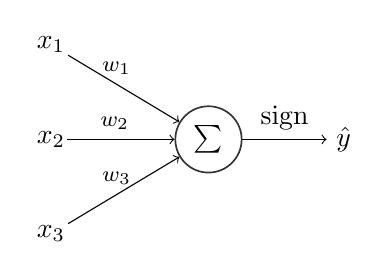
\begin{tikzpicture}
	\tikzstyle{neuron} = [circle,draw=black!80,semithick,minimum size=20pt]
	% input layer
	\foreach \i in {1,...,3}
		\node (input\i) at (0, -\i*1.2) {$x_\i$};
	% perceptron
	\node[neuron] (perceptron) at (2, -2*1.2) {$\sum$};
	% connections
	\foreach \i in {1,...,3}
		\draw[->, shorten <= -.1cm] (input\i) -- node[pos=.4,above]{\footnotesize{$w_\i$}} (perceptron);
	% output
	\draw[->] (perceptron) -- node[above]{$\sign$}(3.5, -2*1.2) node[right]{$\hat{y}$};
\end{tikzpicture}
	\end{center}
	\caption{An illustration of the perceptron model. In this example, the perceptron accepts three inputs $x_1, x_2, x_3$, has the parameters $w_1, w_2, w_3$, and computes $\hat{y} = \sign(w_1x_1 + w_2x_2 + w_3x_3).$}
	\label{fig:perceptron}
\end{figure}

Perceptron models can be used to solve binary classification problems. In this scenario, we are given a list of $m$ training examples $\mathbb{X} = (\bm{x}^{(1)}, \ldots, \bm{x}^{(m)})$ and their corresponding binary labels $\mathbb{Y}$, and wish to predict the most probable label for an unseen vector $\bm{x} \notin \mathbb{X}$.

For example, the vectors $\bm{x}^{(i)}$ might describe features of an email using a \emph{bag-of-words} representation. That is, we define a fixed vocabulary, and the \nth{j} entry in the vector $\bm{x}^{(i)}$ specifies how often the \nth{j} word of the vocabulary occurs in the particular email represented by $\bm{x}^{(i)}$. The corresponding label $y^{(i)} = 1$ then might signify that the email is a legitimate email, whereas a value of $y^{(i)} = -1$ might label the email as spam.

In the beginning, the weights are randomly initialized and the model thus makes arbitrary predictions. During the process of \emph{training} the perceptron, we iteratively adjust the weights in order to improve the prediction accuracy on the training set.

One common method of training is the perceptron learning algorithm proposed by Rosenblatt \cite{Rosenblatt1958386}\DIFdelbegin \DIFdel{. Essentially, the algorithm iterates through the training data $\mathbb{X}$ and makes small adjustments to the weights if a particular training example $\bm{x}^{(i)}$ is misclassified. For example, if the perceptron predicts $\hat{y} = 1$ and the actual label is $y^{(i)} = -1$, the weights are corrected in the negative direction. Since the perceptron learning algorithm }\DIFdelend \DIFaddbegin \DIFadd{, which we will not cover in this paper, since it }\DIFaddend is not directly applicable to neural networks\DIFdelbegin \DIFdel{, we will not discuss it further; a more }\DIFdelend \DIFaddbegin \DIFadd{. An }\DIFaddend in depth explanation can be found in Ref. \cite[Ch.\,8,\,pp.\,265-267]{DBLP:books/lib/Murphy12}.

A major shortcoming of the perceptron is that it can only learn to classify linearly separable data \cite{DBLP:books/daglib/0066902}. For example, the \textsc{xor} function, where 
\begin{equation}
\text{\textsc{xor}}(\bm{x}) = 
\begin{cases} 0 & \text{if }\bm{x} = [0,0] \lor \bm{x} = [1,1] 
			\\1 & \text{if }\bm{x} = [1,0] \lor \bm{x} = [0,1],
\end{cases}
\end{equation}
cannot be learned with the perceptron\DIFaddbegin \DIFadd{, since there exists no linear function that perfectly partitions the data into the two classes $0$ and $1$}\DIFaddend . The discovery of these limitations has greatly reduced interest in the field of biological learning, until more sophisticated models, such as neural networks, were developed \cite[Ch.\,1,\,pp.\,12-18]{DBLP:books/daglib/0040158}.
\section{Feedforward Neural Networks}
\label{sec:feedforward_neural_networks}
A natural extension of the perceptron model is to combine multiple perceptrons in a network architecture called a neural network. It is intuitively clear that, much like in an organic brain, a complex arrangement of many simple computing units can learn much more complicated functions than those simple units alone. In this section, we will examine how such a network architecture based on perceptrons can be constructed. The ideas that we develop are mostly based on Ref. \cite[Ch.\,6]{DBLP:books/daglib/0040158}.

\subsection{Extensions to the Perceptron}
Before explaining the composition of perceptrons to neural networks, we will first explore two common extensions to the perceptron model \DIFdelbegin \DIFdel{, }\DIFdelend which are required in the network architecture we develop.

First, we introduce an additional term called \emph{bias} to the output calculation. The new output $\hat{y}$ becomes
\begin{equation}\label{eq:perceptron2}
\hat{y} = \sign(\bm{w}^\top\bm{x} + b),
\end{equation}
where the scalar $b$ is the bias. This additional learnable parameter shifts the function computed by the model \emph{independently of its input}. \DIFdelbegin \DIFdel{If the bias is large and positive, the model is generally more inclined to predict a positive label, while a negative bias makes it more likely that negative labels are predicted}\DIFdelend \DIFaddbegin \DIFadd{Learning a bias value can therefore help the model make better predictions}\DIFaddend .

Second, we generalize the perceptron by replacing the $\sign$ function with an arbitrary function $f$ called \emph{activation function}. In contrast to $\sign(x)$, most activation functions used in neural networks are continuous, since this enables us to use a variety of \emph{gradient-based} learning algorithms for training as we will see in Section \ref{sec:training}. Concrete examples of activation functions will be discussed later in this section.

We also introduce the quantity $z$, the \emph{weighted input}, which simply is defined as
\begin{equation}\label{eq:perceptron3}
z = \bm{w}^\top\bm{x} + b.
\end{equation}

The computing units we have obtained with these modifications to the perceptron are generally called \emph{neurons} or simply \emph{units}.

\subsection{Network architecture}
Any arrangement of neurons in a network architecture can be considered a neural network. The most influential such architecture is the feedforward neural network, which forms the basis for many other more advanced neural networks \cite[Ch.\,6,\,p.\,163]{DBLP:books/daglib/0040158}. Feedforward neural networks are sometimes also called \emph{multilayer perceptrons} (MLPs).

In feedforward neural networks, the computing units are arranged in layers. We distinguish between the \emph{output layer}, the \emph{hidden layers}, and the \emph{input layer}. The output layer is the final layer in the network were its actual output is produced. The input layer is the first layer in the network, and all layers in between are called hidden layers. The input layer is special in that it does not compute anything; it merely represents the input that is passed into the neural network. In general, a $L$-layer feedforward neural network consists of one input layer, $(L-2)$ hidden layers, and an output layer. We call the number of layers $L$ the \emph{depth} of the model.

Every neuron in a layer $l$ receives input from all neurons in the \nth{(l-1)} layer. There are no connections between neurons in the same layer, and we also do not allow feedback connections into previous layers. Neurons in the hidden and output layers behave exactly like the modified perceptron; the only important detail is that their input is the output from the previous layer. An illustration of a feedforward neural network can be found in Fig. \ref{fig:network}.
\begin{figure}
	\begin{center}
		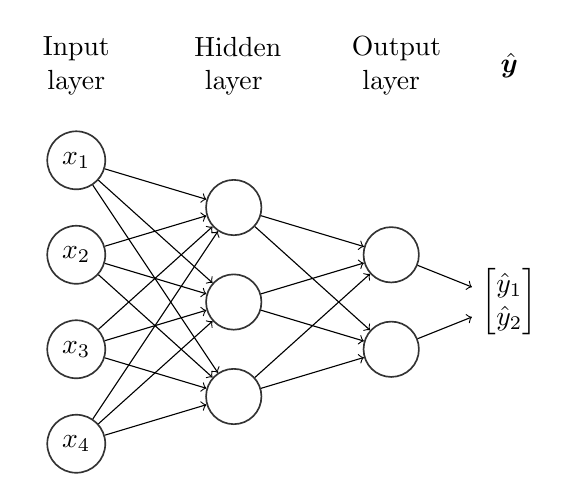
\begin{tikzpicture}
	\tikzstyle{neuron} = [circle,draw=black!80,semithick,minimum size=20pt]
	\tikzstyle{layer} = [text width=1cm, align=center]
	% input layer
	\node[layer] at (0, 0) {Input layer};
	\foreach \i in {1,...,4}
		\node[neuron] (input\i) at (0, -\i*1.2) {$x_\i$};
	% hidden layer
	\node[layer] at (2, 0) {Hidden layer};
	\foreach \i in {1,...,3}
		\node[neuron] (hidden\i) at (2, -\i*1.2 -.6) {};
	% output layer
	\node[layer] at (4, 0) {Output layer};
	\foreach \i in {1,...,2}
		\node[neuron] (output\i) at (4, -\i*1.2 -1.2) {};
	% connections input->hidden
	\foreach \i in {1,...,4}
		\foreach \j in {1,...,3}
			\draw[->] (input\i) -- (hidden\j);
	% connections hidden->output
	\foreach \i in {1,...,3}
		\foreach \j in {1,...,2}
			\draw[->] (hidden\i) -- (output\j);

	\node[layer] at (5.5, 0) {$\hat{\bm{y}}$};
	\node (vec) at (5.5, -1.2 - 1.8) {$\begin{bmatrix}\hat{y}_1\\
		\hat{y}_2\end{bmatrix}$};
	\draw[->] (output1) -- (vec);
	\draw[->] (output2) -- (vec);
\end{tikzpicture}
	\end{center}
	\caption{A three-layer neural network. The network accepts an input $\bm{x} \in \mathbb{R}^4$, propagates it through its hidden layer consisting of three units, and finally produces an output $\hat{\bm{y}} \in \mathbb{R}^2$ in the output layer. The weights, sums, and activation functions have been omitted.}
	\label{fig:network}
\end{figure}

In the remainder of this section, we discuss the individual layers and corresponding design decisions in more detail.

\subsubsection{Output layer}
The design of the output layer depends mostly on the task that we wish to perform with the neural network. 

If we want to predict a numerical value, a problem known as \emph{regression}, we only use a single linear neuron in the output layer. A linear neuron simply uses the identity function as its activation function. \DIFaddbegin \DIFadd{The output of the neural network thus is simply the weighted input of the neuron in the output layer and can cover the whole domain of $\mathbb{R}$. This design can readily be extended to predict a vector of numerical values: we simply use as many linear output neurons as the number of values we want to predict.
}\DIFaddend 

In \emph{classification}, we wish to predict the class of an input vector $\bm{x}$, given a set of classes. For example, as with the perceptron, we might want to distinguish normal emails from spam emails. In this case of \emph{binary} classification, it is common to use the activation function
\begin{equation}
\sigma(x) = \frac1{1+\exp(-x)},
\end{equation}
called the logistic sigmoid, in combination with a single output unit.
\DIFdelbegin %DIFDELCMD < \begin{figure}
%DIFDELCMD < 	\begin{center}
%DIFDELCMD < 		%%%
%DIF <  !TeX root = dm-template.tex
%DIFDELCMD < 

%DIFDELCMD < %%%
%DIF <  restrict y to domain=-1:1, x=1cm
%DIFDELCMD < \begin{tikzpicture}[scale=.9]
%DIFDELCMD < 	\begin{axis}[axis lines = left,xlabel = $x$, ylabel = {$\sigma(x)$}, ymin=-0.05, ymax=1.05]
%DIFDELCMD < 		\addplot [domain=-6:6, samples=200, color=blue, style=semithick]
%DIFDELCMD < 		{1/(1+exp(-x))};
%DIFDELCMD < 		%\addlegendentry{$\sigma(x) = 1/\exp(-x)$}
%DIFDELCMD < 	\end{axis}
%DIFDELCMD < \end{tikzpicture}
%DIFDELCMD < 	\end{center}
%DIFDELCMD < 	%%%
%DIFDELCMD < \caption{%
{%DIFAUXCMD
\DIFdelFL{The logistic sigmoid function.}}
	%DIFAUXCMD
%DIFDELCMD < %DIFDELCMD < \label{fig:sigmoid}%%%
%DIFDELCMD < \end{figure}
%DIFDELCMD < %%%
\DIFdel{As shown in Fig. \ref{fig:sigmoid}, }\DIFdelend %DIF > \begin{figure}
%DIF > 	\begin{center}
%DIF > 		% !TeX root = template_Beamer.tex

% restrict y to domain=-1:1, x=1cm
\begin{tikzpicture}[scale=.9]
	\begin{axis}[axis lines = left,xlabel = $x$, ylabel = {$\sigma(x)$}, ymin=-0.05, ymax=1.05, mlineplot]
		\addplot [domain=-6:6, samples=200,color=blue, style=semithick]
		{1/(1+exp(-x))};
		%\addlegendentry{$\sigma(x) = 1/\exp(-x)$}
	\end{axis}
\end{tikzpicture}
%DIF > 	\end{center}
%DIF > 	\caption{The logistic sigmoid function.}
%DIF > 	\label{fig:sigmoid}
%DIF > \end{figure}
\DIFaddbegin \DIFadd{One can easily see that }\DIFaddend $\sigma(x)$ \DIFaddbegin \DIFadd{behaves like a smoothed version of the $\sign$ function and }\DIFaddend squashes its input to a value between 0 and 1, which can be interpreted as a probability distribution. Thus, it is an excellent choice for binary classification problems: the output $\hat{y}$ of the neural network is the probability that $\bm{x}$ belongs to class 1, while $(1-\hat{y})$ is the probability that $\bm{x}$ belongs to class 0.

In \emph{multiclass} classification problems, where we wish to predict a probability distribution over $k$ different classes, we construct an output layer with $k$ units. A generalization of the logistic sigmoid, called the $\softmax$ function
\begin{equation}\label{eq:softmax}
\softmax(x) = \frac{\exp(x)}{\sum_{i=1}^{k}\exp(z_i)},
\end{equation}
is commonly used as activation function in this scenario. In Eq. \eqref{eq:softmax}, $z_i$ represents the weighted input $z$ of the \nth{i} neuron in the output layer. We can easily see that the $\softmax$ function creates a valid probability distribution and that neurons that have a large weighted input produce a higher probability. The output $\hat{y}_i$ of the neural network is the probability it assigns to the \nth{i} class.

Feedforward neural networks can also be applied to many other tasks such as \emph{structured output prediction}, \emph{anomaly detection}, and \emph{synthesis} \cite[Ch.\,5,\,pp.\,96-100]{DBLP:books/daglib/0040158}. Many specialized architectures exist for these types of problems, but they are beyond the scope of this paper.
\subsubsection{Hidden layers}
In contrast to the output layer, the task that we want so solve does not give us any information about how to design the hidden layers. The first and foremost design decision that comes to mind is the depth of the neural network. 

From a purely theoretical point of view, the depth of a network is irrelevant. It can be shown that a feedforward neural network with just one hidden layer can approximate any function arbitrarily well, given that enough hidden units are available \cite{DBLP:journals/nn/HornikSW89,DBLP:journals/mcss/Cybenko89}. However, this does not mean that we know how to design or train such a network, and deeper networks almost always perform better in practice.

We can think of the hidden layers as a means to learn a different representation of the input. The neural network transforms the input by propagating it through its hidden layers until it obtains a representation where it can perform the assigned task much easier. For example, in object recognition, one can show that neural networks learn to detect different features such as edges or individual object parts in different hidden layers \cite{DBLP:conf/eccv/ZeilerF14}. It is thus not surprising that deeper neural networks \DIFdelbegin \DIFdel{often }\DIFdelend \DIFaddbegin \DIFadd{generally }\DIFaddend perform better than shallow ones. On the other hand, deep neural networks are often difficult and computationally expensive to train.

Another important consideration is the activation function used in hidden layers. Common activation functions include the logistic sigmoid, which we have already presented, the $\tanh$ function, which is only a variation of the logistic sigmoid function, and the rectified linear function $g(x) = \max\{0,x\}$.
%DIF < , a plot of which can be found in Fig. \ref{fig:relu}.
\DIFdelbegin %DIFDELCMD < 

%DIFDELCMD < \begin{comment}
%DIFDELCMD < \begin{figure}
%DIFDELCMD < 	\begin{center}
%DIFDELCMD < 		%%%
%DIF <  !TeX root = dm-template.tex
%DIFDELCMD < 

%DIFDELCMD < %%%
%DIF <  restrict y to domain=-1:1, x=1cm
%DIFDELCMD < \begin{tikzpicture}[scale=.9]
%DIFDELCMD < 	\begin{axis}[axis lines = left,xlabel = $x$, ylabel = {$\max\{0,x\}$}, ymin=-0.5]
%DIFDELCMD < 		\addplot [domain=-8:8, samples=200, color=blue, style=semithick]
%DIFDELCMD < 		{max(0,x)};
%DIFDELCMD < 		%\addlegendentry{$\sigma(x) = 1/\exp(-x)$}
%DIFDELCMD < 	\end{axis}
%DIFDELCMD < \end{tikzpicture}
%DIFDELCMD < 	\end{center}
%DIFDELCMD < 	%%%
%DIFDELCMD < \caption{%
{%DIFAUXCMD
\DIFdelFL{The rectified linear function.}}
	%DIFAUXCMD
%DIFDELCMD < %DIFDELCMD < \label{fig:relu}%%%
%DIFDELCMD < \end{figure}
%DIFDELCMD < \end{comment}
%DIFDELCMD < %%%
\DIFdelend 

Activation functions are continuous, a property needed for the training algorithm, and generally non-linear, since a network consisting of only linear hidden layers is linear as a whole, suffering from the same drawbacks that we saw in the perceptron model \cite[Ch.\,6,\,p.\,190]{DBLP:books/daglib/0040158}.

The design of neural networks is mostly driven by experimentation and not many theoretical tools exist that justify the use of one architecture over another. For example, rectified linear units often outperform other types of hidden units \cite{DBLP:journals/jmlr/GlorotBB11 ,DBLP:conf/nips/KrizhevskySH12}, but we are far from a rigorous understanding of why this is the case. Thus, a network design for a particular task is mostly chosen via trial and error \cite[Ch.\,6,\,pp.\,185-187]{DBLP:books/daglib/0040158}.

\subsubsection{Input layer}
Since the input layer only represents the input passed to the neural network, there are not many design decisions to be made. We can only choose how we wish to represent the input. Often, this representation follows immediately from the raw data--for example, in image classification, we can simply represent an input image as a vector \DIFaddbegin \DIFadd{or tensor }\DIFaddend of pixel values. In other cases, the input representation might not be that obvious and we may need carefully hand-crafted features.

\subsection{Mathematical formulation}
As we have seen, a feedforward neural network is simply a combination of many perceptron-like computing units. We can combine all parameters of these neurons in weight matrices and bias vectors to obtain one single mathematical specification of the whole network.

In particular, we define a weight matrix $\bm{W}^{(l)}$ for every layer $l$ except the input layer, where the entry in the \nth{j} row and \nth{k} column equals the weight of the \nth{j} neuron in the \nth{(l-1)} layer to the \nth{k} neuron in the \nth{l} layer. We specify the entries of the weight matrices with $w_{jk}^{(l)}$. We similarly define bias vectors $\bm{b}^{(l)}$ whose \nth{j} entry contains the bias of the \nth{j} neuron in the \nth{l} layer. We denote the activation function used in the \nth{l} layer with $f^{(l)}$. Activation functions are applied element-wise to vectors.

We can now denote the output $\bm{a}^{(l)}$ of the \nth{l} layer as
\begin{equation}
\bm{a}^{(l)} = f^{(l)}\left(\bm{W}^{(l)\top}\bm{a}^{(l-1)}+\bm{b}^{(l)}\right),
\end{equation}
where $\bm{a}^{(0)} = \bm{x}$. The output of the whole network then is simply given by $\hat{\bm{y}} = \bm{a}^{(L)}$. We also define the vector of weighted inputs $\bm{z}^{(l)}$ at layer $l$ as
\begin{equation}
\bm{z}^{(l)} = \bm{W}^{(l)\top}\bm{a}^{(l-1)}+\bm{b}^{(l)}.
\end{equation}

Note that these expressions are very similar to the formulation of the perceptron model in Eq. \eqref{eq:perceptron2} and \eqref{eq:perceptron3}. The only difference is that we now use matrices, since there are multiple neurons in a layer, and that the total output consists of a chain of multiple such functions.

As shorthand notation, we will sometimes refer to the parameters of a neural network as $\bm{\theta}$ and to the whole neural network as $f(\bm{\theta})$, abstracting away the individual layers.
\begin{comment}
\begin{equation}
f(\bm{x}) = f^{(L)}(\bm{W}^{(L)\top}f^{(L-1)}(\bm{W}^{(L-1)\top}\dotsm+\bm{b}^{(l-1)})+\bm{b}^{(L)}
\end{equation}
\end{comment}
\section{Training Feedforward Neural Networks}
\label{sec:training}
Similar to the perceptron model, when training neural networks, we have a list of $m$ training examples $\mathbb{X} = (\bm{x}^{(1)}, \ldots, \bm{x}^{(m)})$ with corresponding labels $\mathbb{Y}$, and wish to iteratively adjust the parameters $\bm{\theta}$ of the neural network to learn a mapping from $\mathbb{X}$ to $\mathbb{Y}$. The parameters are usually randomly initialized.

In a binary classification setting, the labels $y^{(i)}$ are either 0 or 1 to indicate one of the two classes. In multiclass problems, they encode one of $k$ classes in a \emph{one-hot} fashion: in this case, $\bm{y}^{(i)}$ is a $k$-dimensional vector whose \nth{i} entry is 1 if $\bm{y}^{(i)}$ represents the \nth{i} class. All other entries are equal to 0. Finally, in regression, the labels are simply the \DIFdelbegin \DIFdel{scalar }\DIFdelend values that we want to predict.

Suppose we are given such a set of training data and a neural network $f(\bm{\theta})$. In this section, we explore how we can choose $\bm{\theta}$ in order that the network learns the mapping described by the training data, mainly utilizing concepts presented in Ref. \cite{DBLP:books/daglib/0040158} and \cite{Nielsen2015}.

\DIFaddbegin \DIFadd{We will focus on gradient-based learning, which is the most common method employed in neural networks. Other algorithms, such as genetic algorithms, are also used in special scenarios \mbox{%DIFAUXCMD
\cite{DBLP:conf/ijcai/MontanaD89}}%DIFAUXCMD
, but they are beyond the scope of this paper.
}

\DIFaddend \subsection{Cost functions}
\DIFdelbegin \DIFdel{Since we start with a random set of parameters which we wish to improve , we }\DIFdelend \DIFaddbegin \DIFadd{In order to improve the parameters $\bm{\theta}$, we first }\DIFaddend need some kind of measure of how good the network performs \DIFaddbegin \DIFadd{with those particular parameters}\DIFaddend . For this, we introduce the \emph{cost function} $J(\bm{\theta})$, sometimes also referred to as \emph{loss} or \emph{error} function. $J(\bm{\theta})$ produces a scalar cost \DIFdelbegin \DIFdel{which }\DIFdelend \DIFaddbegin \DIFadd{with two properties: it }\DIFaddend is non-negative and the closer it is to 0, the better our network performs. We can thus reframe the training problem as \emph{minimizing the cost function}.

The cost functions that we will consider can all be represented as sums over the costs of the individual training examples:
\begin{equation}
J(\bm{\theta}) = \frac1{m}\sum_{i=1}^{m}\loss(\bm{x}^{(i)},\bm{y}^{(i)},\bm{\theta}),
\end{equation}
where $\loss$ is the loss for an individual training example. We scale $J$ by $1/m$ to make the cost independent of the number of training examples $m$.

The particular per-example cost function $\loss$ is chosen based on the task that we wish to perform\DIFdelbegin \DIFdel{.
}\DIFdelend \DIFaddbegin \DIFadd{:
}\DIFaddend 

In regression, a good choice is the \emph{mean squared error}
\begin{equation}
\loss(\bm{x}, y, \bm{\theta}) = \frac1{2}(\hat{y}-y)^2,
\end{equation}
which simply corresponds to the distance of the desired output $y$ from the actual output $\hat{y}$. It can easily be seen that it satisfies the properties of a cost function: it is always non-negative and if $\hat{y}$ is similar to $y$, then $(\hat{y}-y)^2/2 \approx 0$.

The mean squared error is also a valid cost function in  binary classification problems. However, it has some undesirable properties that can make training \DIFdelbegin \DIFdel{very }\DIFdelend difficult in this setting\DIFaddbegin \DIFadd{. In particular, the gradient of the mean squared error can become very small in combination with sigmoid neurons, which causes the network to only learn slowly as we will see later in this section }\DIFaddend \cite[Ch.\,6,\,p.\,178]{DBLP:books/daglib/0040158}. Hence, a different cost function, called the \emph{cross-entropy}, is commonly chosen. The cross-entropy loss is defined as
\begin{equation}
\loss(\bm{x}, y, \bm{\theta}) = -y \ln \hat{y} - (1-y)\ln(1-\hat{y}).
\end{equation}
We observe that, if $y=1$, the loss simply becomes $-\ln\hat{y}$, which is large if $\hat{y}$ is close to 0, and small if $\hat{y}$ is close to 1. A similar analysis can be conducted for the case $y=0$ and we can see that this cost function also satisfies the desired properties.

In case of multiclass classification, the cross-entropy becomes
\begin{equation}
\loss(\bm{x}, \bm{y}, \bm{\theta}) = -\ln \hat{y}_i
\end{equation}
if $\bm{y}$ represents the \nth{i} class (i.e. the \nth{i} position in the vector $\bm{y}$ is 1). Similar arguments as in the case of binary classification apply as to why this is a valid cost function.

While these functions might seem rather different, they can all be derived with the same principle, called \emph{maximum likelihood estimation} (MLE) \cite[Ch.\,5,\,pp.\,128-131]{DBLP:books/daglib/0040158}. This estimation comes from a probabilistic perspective and interprets the training data as samples drawn from an unknown probability distribution $P(\mathbb{Y}\given\mathbb{X})$. From this perspective, the goal of training is to choose parameters $\bm{\theta}$ such that the probability distribution $P_{\text{model}}(\mathbb{Y}\given\mathbb{X}; \bm{\theta})$ described by the model matches the true distribution as closely as possible. The MLE states that we should choose the parameters that maximize $P_{\text{model}}$, i.e. the optimal parameters $\hat{\bm{\theta}}$ are
\begin{equation}
\hat{\bm{\theta}} = \argmax_{\bm{\theta}} P_{\text{model}}(\mathbb{Y}\given\mathbb{X}; \bm{\theta}).
\end{equation}

We obtain the mean squared error from the MLE if we regard the true probability distribution of the data as a Gaussian distribution. In the case of binary and multiclass classification, we regard the true probability distribution as a Bernoulli or Multinoulli distribution, respectively \cite[Ch.\,6,\,pp.\,175-185]{DBLP:books/daglib/0040158}.

\subsection{Stochastic Gradient Descent}
Minimizing cost functions is similar to any other minimization problem. A variety of algorithms exist to minimize functions, but stochastic gradient descent, an extension of gradient descent, is particularly dominant in neural network training\DIFaddbegin \DIFadd{, because it is rather efficient and yields good results}\DIFaddend .

As the name suggests, gradient descent makes use of the gradient of the cost function to iteratively improve the parameters to decrease the cost. In particular, we know from calculus that a small change $\Delta\bm{\theta}$ in $\bm{\theta}$ corresponds roughly to the change
\begin{equation}
\Delta J(\bm{\theta}) \approx \nabla J(\bm{\theta})^{\top}\Delta\bm{\theta}
\end{equation}
in $J(\bm{\theta})$. It can be shown that the choice of $\Delta\bm{\theta}$ which decreases the cost the fastest and thus minimizes $\Delta J(\bm{\theta})$ is
\begin{equation}
\Delta\bm{\theta} = -\eta\nabla J(\bm{\theta}),
\end{equation}
where $\eta$ is the \emph{learning rate} \cite[Ch.\,4,\,p.\,82]{DBLP:books/daglib/0040158}. This means that we can improve a neural network by making small changes to the parameters in the negative direction of the gradient of the cost function.

The learning rate $\eta$ controls the size of the update steps performed by gradient descent. It should neither be too small, nor too large: if it is small, the model only learns very slowly, and if it is large, we risk making updates that unintentionally increase the loss, since the gradient is only an approximation of the real cost function.

The problem with using gradient descent to train neural networks is that computing the gradient is linear in the number of training examples $m$. To see this, note that
\begin{equation}
\nabla J(\bm{\theta}) = \frac1{m}\sum_{i=1}^{m}\nabla \loss(\bm{x}^{(i)},\bm{y}^{(i)},\bm{\theta}).
\end{equation}
\emph{Stochastic} gradient descent resolves this dependency by computing an approximation of the gradient by averaging over only a subset of training examples with corresponding labels $\mathbb{B}$ called a \emph{minibatch}. The gradient computation becomes
\begin{equation}
\nabla J(\bm{\theta}) = \frac1{|\mathbb{B}|}\sum_{(\bm{x},\bm{y})\in\mathbb{B}}\nabla \loss(\bm{x},\bm{y},\bm{\theta}),
\end{equation}
which is independent of $m$. The size $|\mathbb{B}|$ of the minibatches is not increased with the amount of training data.

Many variations of stochastic gradient descent exist. They usually make use of higher order derivatives or approximations thereof and dynamically adjust the learning rate \cite{DBLP:journals/corr/Ruder16}.

\subsection{The Back-propagation Algorithm}
An efficient way of computing the gradient of the cost function is the back-propagation algorithm \cite{Rumelhart1986533}. Beginning from the output layer, the algorithm computes the partial derivatives of all the weights and biases up to the first hidden layer. In the remainder of this section, we derive this procedure mathematically and show how it can be used in combination with stochastic gradient descent to train feedforward neural networks. \DIFdelbegin \DIFdel{We assume familiarity with basic multivariable calculus. }\DIFdelend The derivation we present is closely based on Ref. \cite[Ch.\,2]{Nielsen2015}.

The ultimate goal of the algorithm is to compute the partial derivatives $\partial J/\partial w_{ij}^{(l)}$ and $\partial J/\partial b_j^{(l)}$. To achieve this, we introduce the intermediate quantity
\begin{equation}
\delta_j^{(l)} = \frac{\partial J}{\partial z_j^{(l)}},
\end{equation}
which is a measure of the error in the \nth{j} neuron of the \nth{l} layer: if $\delta_j^{(l)}$ is large, changing the parameters of this neuron can decrease the cost considerably, and if it is small, the neuron is already near-optimal. The error is closely related to the quantities of interest: with the chain rule, we obtain
\begin{equation}\label{eq:bp1}
\frac{\partial J}{\partial b_j^{(l)}}
= \frac{\partial J}{\partial z_j^{(l)}}\frac{\partial z_j^{(l)}}{\partial b_j^{(l)}}
= \delta_j^{(l)} \frac{\partial\left (\sum_{i}w_{ij}^{(l)}a_i^{(l-1)} + b_j^{(l)}\right)}{\partial b_j^{(l)}}
= \delta_j^{(l)},
\end{equation}
and similarly,
\begin{equation}\label{eq:bp2}
\frac{\partial J}{\partial w_{ij}^{(l)}}
= \frac{\partial J}{\partial z_j^{(l)}}\frac{\partial z_j^{(l)}}{\partial w_{ij}^{(l)}}
= \delta_j^{(l)} \frac{\partial z_j^{(l)}}{\partial w_{ij}^{(l)}}
= \delta_j^{(l)}a_i^{(l-1)}.
\end{equation}
We can arrange those derivatives in vectors and matrices matching the bias vectors and weight matrices in dimension. The bias derivative vector is simply given by $\bm{\delta}^{(l)}$ and the matrix of weight derivatives is $\bm{a}^{(l-1)}\bm{\delta}^{(l)\top}$. \DIFaddbegin \DIFadd{This enables us to formulate the parameter update of stochastic gradient descent as a single subtraction of the derivative matrix from the corresponding weight matrix.
}\DIFaddend 

All that remains is the calculation of $\bm{\delta}^{(l)}$ itself. We start with the output layer $L$:
\begin{equation}
\delta_j^{(L)} = \frac{\partial J}{\partial z_j^{(L)}}
= \frac{\partial J}{\partial \hat{y}_j} \frac{\partial \hat{y}_j}{\partial z_j^{(L)}}
= \frac{\partial J}{\partial \hat{y}_j} f^{(L)\prime}\left (z_j^{(L)}\right ),
\end{equation}
which, in vector notation, becomes
\begin{equation}
\bm{\delta}^{(L)} = \nabla_{\hat{\bm{y}}}J \odot f^{(L)\prime}\left (\bm{z}^{(L)}\right ).
\end{equation}
Here, $\bm{x} \odot \bm{y}$ denotes the entry-wise product between $\bm{x}$ and $\bm{y}$.

Finally, the output error can be propagated back to earlier layers. Again applying the chain rule,
\begin{equation}
\delta_j^{(l)} = \frac{\partial J}{\partial z_j^{(l)}}
= \sum_k \frac{\partial J}{\partial z_k^{(l+1)}} \frac{\partial z_k^{(l+1)}}{\partial z_j^{(l)}}
= \sum_k \delta_k^{(l+1)} \frac{\partial z_k^{(l+1)}}{\partial z_j^{(l)}},
\end{equation}
where the sum is over all neurons in the \nth{(l+1)} layer. Note that
\begin{equation}
\begin{gathered}
\frac{\partial z_k^{(l+1)}}{\partial z_j^{(l)}}
= \frac{\partial\left (
	\sum_j w_{jk}^{(l+1)}f^{(l)}\left (z_j^{(l)}\right )+b_k^{(l+1)}
	\right )}{\partial z_j^{(l)}}\\
= w_{jk}^{(l+1)}f^{(l)\prime}\left (z_j^{(l)}\right ).
\end{gathered}
\end{equation}
Substituting back, we obtain
\begin{equation}
\delta_j^{(l)} = \sum_k \delta_k^{(l+1)} w_{jk}^{(l+1)}f^{(l)\prime}\left (z_j^{(l)}\right ),
\end{equation}
which is easily expressed in matrix notation:
\begin{equation}\label{eq:bp3}
\bm{\delta}^{(l)} = \bm{W}^{(l+1)} \bm{\delta}^{(l+1)} \odot f^{(l)\prime}\left (\bm{z}^{(l)}\right ).
\end{equation}

These expressions allow for a very efficient computation of the gradient. First, we propagate the input vector of a particular training example forward through the network to obtain the output $\hat{\bm{y}}$. From this, we can calculate the cost $J(\bm{\theta})$ and the error $\bm{\delta}^{(L)}$ in the output layer. With Eq. \eqref{eq:bp3}, the error is then propagated backwards through the hidden layers, where we can easily compute the derivatives using Eq. \eqref{eq:bp1} and \eqref{eq:bp2}.

Combining back-propagation with stochastic gradient descent yields the complete learning algorithm for feedforward neural networks, which is formalized in algorithm \ref{alg:learning} \cite[Ch.\,2]{Nielsen2015},\cite[Ch.\,6,\,pp.\,205-206]{DBLP:books/daglib/0040158}.

\begin{algorithm}
	\caption{The learning algorithm for feedforward neural networks. The algorithm computes one stochastic gradient descent update, given a minibatch $\mathbb{B}$.}
	\begin{algorithmic}
		\Require{A minibatch of training examples $\mathbb{B}$}
		\Require{The model composed of weight matrices $\bm{W}^{(i)}$, bias vectors $\bm{b}^{(i)}$, and activation functions $f^{(i)}$}
		\Require{The learning rate $\eta$}
		\For{$(\bm{x}, \bm{y}) \in \mathbb{B}$}
		\State{$\bm{a}^{(\bm{x},1)} = \bm{x}$}
		\For{$l = 2,\ldots,L$}\Comment{forward propagation}
		\State{$\bm{z}^{(\bm{x},l)} = \bm{W}^{(l)\top}\bm{a}^{(\bm{x},l-1)} + \bm{b}^{(l)}$}
		\State{$\bm{a}^{(\bm{x},l)} = f^{(l)}\left (\bm{z}^{(\bm{x},l)}\right )$}
		\EndFor
		\State{$\hat{\bm{y}} = \bm{a}^{(\bm{x}, L)}$}
		\State{$\bm{\delta}^{(\bm{x},L)} = \nabla_{\hat{\bm{y}}}J \odot f^{(L)\prime}\left (\bm{z}^{(\bm{x},L)}\right )$}
		\For{$l = L-1, \ldots, 2$} \Comment{back-propagation}
		\State{$\bm{\delta}^{(\bm{x},l)} = \bm{W}^{(l+1)} \bm{\delta}^{(\bm{x},l+1)} \odot f^{(l)\prime}\left (\bm{z}^{(\bm{x},l)}\right )$}
		\EndFor
		\EndFor
		\For{$l = L, \ldots, 2$}\Comment{gradient descent}
		\State{$\bm{W}^{(l)} = \bm{W}^{(l)} - \frac{\eta}{|\mathbb{B}|} \sum_{(\bm{x}, \bm{y}) \in \mathbb{B}} \bm{a}^{(\bm{x},l-1)}\bm{\delta}^{(\bm{x},l)\top}$}
		\State{$\bm{b}^{(l)} = \bm{b}^{(l)} - \frac{\eta}{|\mathbb{B}|} \sum_{(\bm{x}, \bm{y}) \in \mathbb{B}}
			\bm{\delta}^{(\bm{x}, l)}$}
		\EndFor
	\end{algorithmic}
	\label{alg:learning}
\end{algorithm}

\begin{comment}
The back-propagation equations give us some insight into why training sometimes is difficult. For example, if we choose the logistic sigmoid function as activation function for a particular hidden layer, we can see from Eq. \eqref{eq:bp3} that the error is multiplied with $\sigma'\left (\bm{z}^{(l)}\right )$. Since the logistic sigmoid function gets very flat for input of large absolute value, its gradient is close to 0 for such inputs. If the gradient is near 0, the update steps of stochastic gradient descent become very small, and the network thus learns slowly
 \cite[Ch.\,6,\,p.\,189]{DBLP:books/daglib/0040158}.
\end{comment}
%\section{Universal Approximation Capabilities}
\label{sec:approximation}

\section{Extensions}
\label{sec:extensions}
The basic feedforward neural networks we have discussed so far \DIFdelbegin \DIFdel{are rarely used in practice. However, they }\DIFdelend form the foundation for a variety of more sophisticated models, which \DIFdelbegin \DIFdel{we briefly examine in this section}\DIFdelend \DIFaddbegin \DIFadd{are more often used in practice. In this section, we briefly examine those extensions of feedforward neural networks}\DIFaddend .

In computer vision, the most common type of neural networks are \emph{convolutional neural networks} \cite{LeCun1989}. These models have been explicitly designed to exploit the spatial structure of images. For example, they \DIFdelbegin \DIFdel{can easily }\DIFdelend \DIFaddbegin \DIFadd{share weights across different neurons, so that they can }\DIFaddend detect the same feature in different parts of an image. \DIFdelbegin \DIFdel{Convolutional }\DIFdelend \DIFaddbegin \DIFadd{Because of their structure, convolutional }\DIFaddend neural networks also require far less parameters than traditional feedforward neural networks and are thus much more efficient to train and evaluate.

\emph{Recurrent neural networks} \cite{Rumelhart1986533} are neural networks that can process sequential data such as natural language and speech. In contrast to feedforward networks, they allow feedback connections from a layer into previous layers. Therefore, the output at a particular step $t$ in a sequence $\bm{x}^{(1)}, \ldots, \bm{x}^{(\tau)}$ depends not only on the input $\bm{x}^{(t)}$, but also on all \DIFdelbegin \DIFdel{the }\DIFdelend previous inputs $\bm{x}^{(1)}, \ldots, \bm{x}^{(t-1)}$. For example, if a recurrent neural network predicts the meaning of a word in a sentence, it can take into account the previous words in the sentence.

While convolutional and recurrent neural networks are the most common extensions of feedforward neural networks, many other specialized networks exist. Neural networks have been adapted to almost every task in machine learning and continue to produce excellent results \cite[Ch.\,5,\,pp.\,96-100]{DBLP:books/daglib/0040158}.
\section{Conclusion}
\label{sec:conclusion}
We have discussed neural networks, a biologically inspired computing model that dominates modern machine learning. Neural networks are complex networks of simple units which are arranged in a layered architecture. By propagating an input through its layers, a neural network can make sophisticated predictions, such as which class the input is most likely to belong to.

Feedforward neural networks can be represented as a chain of matrix operations and applications of nonlinear functions. The parameters of the model are chosen during training, where a cost function that measures the performance of the network is minimized. The most common algorithm to achieve this is stochastic gradient descent, which requires the computation of the gradient of the cost function. This is efficiently handled by the back-propagation algorithm.

\DIFdelbegin %DIFDELCMD < \begin{comment}
%DIFDELCMD < %%%
\DIFdelend Deep learning, the branch of machine learning that is concerned with the development of deep neural networks, has enabled an outstanding amount of advances in the field. \DIFdelbegin %DIFDELCMD < \end{comment}
%DIFDELCMD < %%%
\DIFdel{We believe }\DIFdelend \DIFaddbegin \DIFadd{We expect }\DIFaddend that, with ever-increasing datasets and computational power, as well as the development of more complex and refined models, neural networks will continue to have a great impact on technology and will power more and more intelligent systems in the future.

%%%%%%%%%%%%%%%%%%%%%%%%%%%%%%%%%%%%%%%%%%%%%%%%%%%%%%%%%%%%%%%%%%%%%%%%%%
% 	Acknowledgements
%%%%%%%%%%%%%%%%%%%%%%%%%%%%%%%%%%%%%%%%%%%%%%%%%%%%%%%%%%%%%%%%%%%%%%%%%%

%\section*{Acknowledgment}
%\addcontentsline{toc}{section}{Acknowledgment}

%%%%%%%%%%%%%%%%%%%%%%%%%%%%%%%%%%%%%%%%%%%%%%%%%%%%%%%%%%%%%%%%%%%%%%%%%%
% 	References
%%%%%%%%%%%%%%%%%%%%%%%%%%%%%%%%%%%%%%%%%%%%%%%%%%%%%%%%%%%%%%%%%%%%%%%%%%

% trigger a \newpage just before the given reference
% number - used to balance the columns on the last page
% adjust value as needed - may need to be readjusted if
% the document is modified later
\IEEEtriggeratref{11}
% The "triggered" command can be changed if desired:
%\IEEEtriggercmd{\enlargethispage{-5in}}

% references section
% NOTE: BibTeX documentation can be easily obtained at:
% http://www.ctan.org/tex-archive/biblio/bibtex/contrib/doc/

% can use a bibliography generated by BibTeX as a .bbl file
% standard IEEE bibliography style from:
% http://www.ctan.org/tex-archive/macros/latex/contrib/supported/IEEEtran/bibtex
\bibliographystyle{IEEEtran}
% argument is your BibTeX string definitions and bibliography database(s)
% Generated by IEEEtran.bst, version: 1.13 (2008/09/30)
\begin{thebibliography}{10}
\providecommand{\url}[1]{#1}
\csname url@samestyle\endcsname
\providecommand{\newblock}{\relax}
\providecommand{\bibinfo}[2]{#2}
\providecommand{\BIBentrySTDinterwordspacing}{\spaceskip=0pt\relax}
\providecommand{\BIBentryALTinterwordstretchfactor}{4}
\providecommand{\BIBentryALTinterwordspacing}{\spaceskip=\fontdimen2\font plus
\BIBentryALTinterwordstretchfactor\fontdimen3\font minus
  \fontdimen4\font\relax}
\providecommand{\BIBforeignlanguage}[2]{{%
\expandafter\ifx\csname l@#1\endcsname\relax
\typeout{** WARNING: IEEEtran.bst: No hyphenation pattern has been}%
\typeout{** loaded for the language `#1'. Using the pattern for}%
\typeout{** the default language instead.}%
\else
\language=\csname l@#1\endcsname
\fi
#2}}
\providecommand{\BIBdecl}{\relax}
\BIBdecl

\bibitem{DBLP:journals/ijcv/RussakovskyDSKS15}
\BIBentryALTinterwordspacing
O.~Russakovsky, J.~Deng, H.~Su, J.~Krause, S.~Satheesh, S.~Ma, Z.~Huang,
  A.~Karpathy, A.~Khosla, M.~S. Bernstein, A.~C. Berg, and F.~Li, ``Imagenet
  large scale visual recognition challenge,'' \emph{International Journal of
  Computer Vision}, vol. 115, no.~3, pp. 211--252, 2015. [Online]. Available:
  \url{https://doi.org/10.1007/s11263-015-0816-y}
\BIBentrySTDinterwordspacing

\bibitem{DBLP:conf/iccv/HeZRS15}
\BIBentryALTinterwordspacing
K.~He, X.~Zhang, S.~Ren, and J.~Sun, ``Delving deep into rectifiers: Surpassing
  human-level performance on imagenet classification,'' in \emph{2015 {IEEE}
  International Conference on Computer Vision, {ICCV} 2015, Santiago, Chile,
  December 7-13, 2015}.\hskip 1em plus 0.5em minus 0.4em\relax {IEEE} Computer
  Society, 2015, pp. 1026--1034. [Online]. Available:
  \url{https://doi.org/10.1109/ICCV.2015.123}
\BIBentrySTDinterwordspacing

\bibitem{DBLP:conf/sigir/SeverynM15a}
\BIBentryALTinterwordspacing
A.~Severyn and A.~Moschitti, ``Twitter sentiment analysis with deep
  convolutional neural networks,'' in \emph{Proceedings of the 38th
  International {ACM} {SIGIR} Conference on Research and Development in
  Information Retrieval, Santiago, Chile, August 9-13, 2015}, R.~A.
  Baeza{-}Yates, M.~Lalmas, A.~Moffat, and B.~A. Ribeiro{-}Neto, Eds.\hskip 1em
  plus 0.5em minus 0.4em\relax {ACM}, 2015, pp. 959--962. [Online]. Available:
  \url{http://doi.acm.org/10.1145/2766462.2767830}
\BIBentrySTDinterwordspacing

\bibitem{DBLP:journals/taslp/MohamedDH12}
\BIBentryALTinterwordspacing
A.~Mohamed, G.~E. Dahl, and G.~E. Hinton, ``Acoustic modeling using deep belief
  networks,'' \emph{{IEEE} Trans. Audio, Speech {\&} Language Processing},
  vol.~20, no.~1, pp. 14--22, 2012. [Online]. Available:
  \url{https://doi.org/10.1109/TASL.2011.2109382}
\BIBentrySTDinterwordspacing

\bibitem{DBLP:conf/cvpr/GatysEB16}
\BIBentryALTinterwordspacing
L.~A. Gatys, A.~S. Ecker, and M.~Bethge, ``Image style transfer using
  convolutional neural networks,'' in \emph{2016 {IEEE} Conference on Computer
  Vision and Pattern Recognition, {CVPR} 2016, Las Vegas, NV, USA, June 27-30,
  2016}.\hskip 1em plus 0.5em minus 0.4em\relax {IEEE} Computer Society, 2016,
  pp. 2414--2423. [Online]. Available:
  \url{https://doi.org/10.1109/CVPR.2016.265}
\BIBentrySTDinterwordspacing

\bibitem{DBLP:journals/pami/KarpathyF17}
\BIBentryALTinterwordspacing
A.~Karpathy and L.~Fei{-}Fei, ``Deep visual-semantic alignments for generating
  image descriptions,'' \emph{{IEEE} Trans. Pattern Anal. Mach. Intell.},
  vol.~39, no.~4, pp. 664--676, 2017. [Online]. Available:
  \url{https://doi.org/10.1109/TPAMI.2016.2598339}
\BIBentrySTDinterwordspacing

\bibitem{DBLP:journals/nature/MnihKSRVBGRFOPB15}
\BIBentryALTinterwordspacing
V.~Mnih, K.~Kavukcuoglu, D.~Silver, A.~A. Rusu, J.~Veness, M.~G. Bellemare,
  A.~Graves, M.~A. Riedmiller, A.~Fidjeland, G.~Ostrovski, S.~Petersen,
  C.~Beattie, A.~Sadik, I.~Antonoglou, H.~King, D.~Kumaran, D.~Wierstra,
  S.~Legg, and D.~Hassabis, ``Human-level control through deep reinforcement
  learning,'' \emph{Nature}, vol. 518, no. 7540, pp. 529--533, 2015. [Online].
  Available: \url{https://doi.org/10.1038/nature14236}
\BIBentrySTDinterwordspacing

\bibitem{DBLP:books/daglib/0040158}
\BIBentryALTinterwordspacing
I.~J. Goodfellow, Y.~Bengio, and A.~C. Courville, \emph{Deep Learning}, ser.
  Adaptive computation and machine learning.\hskip 1em plus 0.5em minus
  0.4em\relax {MIT} Press, 2016. [Online]. Available:
  \url{http://www.deeplearningbook.org/}
\BIBentrySTDinterwordspacing

\bibitem{McCulloch1943115}
\BIBentryALTinterwordspacing
W.~McCulloch and W.~Pitts, ``A logical calculus of the ideas immanent in
  nervous activity,'' \emph{The Bulletin of Mathematical Biophysics}, vol.~5,
  no.~4, pp. 115--133, 1943. [Online]. Available:
  \url{https://www.scopus.com/inward/record.uri?eid=2-s2.0-51249194645&doi=10.1007%2fBF02478259&partnerID=40&md5=edb67afceee33d22eaabbf1f8c1dca90}
\BIBentrySTDinterwordspacing

\bibitem{Rosenblatt1958386}
\BIBentryALTinterwordspacing
F.~Rosenblatt, ``The perceptron: A probabilistic model for information storage
  and organization in the brain,'' \emph{Psychological Review}, vol.~65, no.~6,
  pp. 386--408, 1958. [Online]. Available:
  \url{https://www.scopus.com/inward/record.uri?eid=2-s2.0-11144273669&doi=10.1037%2fh0042519&partnerID=40&md5=f6ad02750f121e6d5d33566003d5ac8b}
\BIBentrySTDinterwordspacing

\bibitem{DBLP:books/lib/Murphy12}
K.~P. Murphy, \emph{Machine learning - a probabilistic perspective}, ser.
  Adaptive computation and machine learning series.\hskip 1em plus 0.5em minus
  0.4em\relax {MIT} Press, 2012.

\bibitem{DBLP:books/daglib/0066902}
M.~Minsky and S.~Papert, \emph{Perceptrons - an introduction to computational
  geometry}.\hskip 1em plus 0.5em minus 0.4em\relax {MIT} Press, 1987.

\bibitem{DBLP:journals/nn/HornikSW89}
\BIBentryALTinterwordspacing
K.~Hornik, M.~B. Stinchcombe, and H.~White, ``Multilayer feedforward networks
  are universal approximators,'' \emph{Neural Networks}, vol.~2, no.~5, pp.
  359--366, 1989. [Online]. Available:
  \url{https://doi.org/10.1016/0893-6080(89)90020-8}
\BIBentrySTDinterwordspacing

\bibitem{DBLP:journals/mcss/Cybenko89}
\BIBentryALTinterwordspacing
G.~Cybenko, ``Approximation by superpositions of a sigmoidal function,''
  \emph{{MCSS}}, vol.~2, no.~4, pp. 303--314, 1989. [Online]. Available:
  \url{https://doi.org/10.1007/BF02551274}
\BIBentrySTDinterwordspacing

\bibitem{DBLP:conf/eccv/ZeilerF14}
\BIBentryALTinterwordspacing
M.~D. Zeiler and R.~Fergus., ``Visualizing and understanding convolutional
  networks,'' in \emph{Computer Vision - {ECCV} 2014 - 13th European
  Conference, Zurich, Switzerland, September 6-12, 2014, Proceedings, Part
  {I}}, ser. Lecture Notes in Computer Science, D.~J. Fleet, T.~Pajdla,
  B.~Schiele, and T.~Tuytelaars, Eds., vol. 8689.\hskip 1em plus 0.5em minus
  0.4em\relax Springer, 2014, pp. 818--833. [Online]. Available:
  \url{https://doi.org/10.1007/978-3-319-10590-1_53}
\BIBentrySTDinterwordspacing

\bibitem{DBLP:journals/jmlr/GlorotBB11}
\BIBentryALTinterwordspacing
X.~Glorot, A.~Bordes, and Y.~Bengio, ``Deep sparse rectifier neural networks,''
  in \emph{Proceedings of the Fourteenth International Conference on Artificial
  Intelligence and Statistics, {AISTATS} 2011, Fort Lauderdale, USA, April
  11-13, 2011}, ser. {JMLR} Proceedings, G.~J. Gordon, D.~B. Dunson, and
  M.~Dud{\'{\i}}k, Eds., vol.~15.\hskip 1em plus 0.5em minus 0.4em\relax
  JMLR.org, 2011, pp. 315--323. [Online]. Available:
  \url{http://www.jmlr.org/proceedings/papers/v15/glorot11a/glorot11a.pdf}
\BIBentrySTDinterwordspacing

\bibitem{DBLP:conf/nips/KrizhevskySH12}
\BIBentryALTinterwordspacing
A.~Krizhevsky, I.~Sutskever, and G.~E. Hinton, ``Imagenet classification with
  deep convolutional neural networks,'' in \emph{Advances in Neural Information
  Processing Systems 25: 26th Annual Conference on Neural Information
  Processing Systems 2012. Proceedings of a meeting held December 3-6, 2012,
  Lake Tahoe, Nevada, United States.}, P.~L. Bartlett, F.~C.~N. Pereira,
  C.~J.~C. Burges, L.~Bottou, and K.~Q. Weinberger, Eds., 2012, pp. 1106--1114.
  [Online]. Available:
  \url{http://papers.nips.cc/paper/4824-imagenet-classification-with-deep-convolutional-neural-networks}
\BIBentrySTDinterwordspacing

\bibitem{Nielsen2015}
\BIBentryALTinterwordspacing
M.~A. Nielsen, \emph{Neural Networks and Deep Learning}.\hskip 1em plus 0.5em
  minus 0.4em\relax Determination Press, 2015. [Online]. Available:
  \url{http://neuralnetworksanddeeplearning.com/}
\DIFaddbegin \BIBentrySTDinterwordspacing

\bibitem{DBLP:conf/ijcai/MontanaD89}
\BIBentryALTinterwordspacing
\BIBentrySTDinterwordspacing

\bibitem{DBLP:journals/corr/Ruder16}
\BIBentryALTinterwordspacing
S.~Ruder, ``An overview of gradient descent optimization algorithms,''
  \emph{CoRR}, vol. abs/1609.04747, 2016. [Online]. Available:
  \url{http://arxiv.org/abs/1609.04747}
\BIBentrySTDinterwordspacing

\bibitem{Rumelhart1986533}
\BIBentryALTinterwordspacing
D.~Rumelhart, G.~Hinton, and R.~Williams, ``Learning representations by
  back-propagating errors,'' \emph{Nature}, vol. 323, no. 6088, pp. 533--536,
  1986. [Online]. Available:
  \url{https://www.scopus.com/inward/record.uri?eid=2-s2.0-0022471098&doi=10.1038%2f323533a0&partnerID=40&md5=2e1eae82a89c7503560b15a74e4c698d}
\BIBentrySTDinterwordspacing

\bibitem{LeCun1989}
Y.~LeCun, ``Generalization and network design strategies,'' University of
  Toronto, Tech. Rep. CRG-TR-89-4, 1989.

\end{thebibliography}

%
% <OR> manually copy in the resultant .bbl file
% set second argument of \begin to the number of references
% (used to reserve space for the reference number labels box)
%\begin{thebibliography}{1}
%
%\bibitem{ref:kopka}
%H.~Kopka and P.~W. Daly, \emph{A Guide to {\LaTeX}}, 3rd~ed.\hskip 1em plus
%  0.5em minus 0.4em\relax Harlow, England: Addison-Wesley, 1999.
%
%\end{thebibliography}

%%%%%%%%%%%%%%%%%%%%%%%%%%%%%%%%%%%%%%%%%%%%%%%%%%%%%%%%%%%%%%%%%%%%%%%%%%
% 	End of the document
%%%%%%%%%%%%%%%%%%%%%%%%%%%%%%%%%%%%%%%%%%%%%%%%%%%%%%%%%%%%%%%%%%%%%%%%%%

\end{document}


